\documentclass{article}
\usepackage{bm}
\usepackage{CJK}
\usepackage[ruled,linesnumbered]{algorithm2e}
\usepackage{graphicx,subfig}
\usepackage{latexsym}

\usepackage{xcolor}

\newcommand{\blue}[1]{\textcolor{blue}{#1}}

\begin{document}
    The computation complexity of Nodetermine B{\"{u}}chi Automaton(NBA) has always been a problem for applications. 
    So there are many effort attempt to simplify the NBA and do find some methods. One of the technique called \emph{Partial Order Reduction} is to reduce the number of possible orderings that need to be analyzed for checking formule stated in  a temporal logic as LTL.  The main purpose is to reduce the state space of the transition system and there are some differece between Computer Science and Multi-agent system technically. The former use it to find a reduced system consists of a single path while the latter want to find all the Partial Order without loose much message.

\blue{There are many typos in the documents. Use a spell-checker in the editor.}
    
    
    Given a Linear Temporal Logic(LTL) formula, we can use the existing tools such as LTL2BA to construt the NBA $A_\phi=(\nu,\varepsilon)$ (which can also be defined as a tuple $\mathcal{B}=(Q_B,Q^0_B,\Sigma,\rightarrow_B,Q^F_B)$).
    Before consider the product with Transition System(TS) of Multi-agents, we only use the message within the NBA $A_\phi$ to get the sets of posets $P_\phi$ for simplification. It worth noting that $P_\phi$ is no longer a Graph and we only use it for the further computation with $TS$. 

\blue{Add proper definition of $\mathcal{B}$ here, i.e., with all the elements property defined.}

\blue{Use section...not bold. Follow a simple \LaTeX tutorial.}


    \textbf{A.Trimming the NBA}
     
    We only consider the \emph{disjunctive normal form} (DNF) $A_{DNF}$ of $A_\phi$ with the assumption that a optimal run in Buchi should not wasted cost at any node's self loop. Then, to trimming the useless edges, we defined the  triangle property as definition 1.1. Once any three vertices $v_1,v_2,v_3$ in $A_{DNF}$ 
    satisfied the RT property, we can remove the edge $\epsilon_{13}$ while the feasibility of $A_{DNF}$ would not be compromised. With a little abuse of notation, we call the NBA $A^-$ after $A_{DNF}$ been processed by RT property. 
     
\blue{DNF of a NBA is equivalent to the original NBA. Namely, there is no simplification when using DNF.}

\blue{Do not use explicit enumeration. Use environment and references.}

    Definition 1.1:(Redundance triangle property) Given three different vertices $v_1,v_2,v_s$ in the $A_{DNF}$. . The function $L(\epsilon)$ means get the labels in the edge $\epsilon$. we say that these three vertices satifsfy the RT property if:
     
    (a)   $\epsilon_{12}=v_1\rightarrow v_2,\epsilon_{23}=v_2\rightarrow v_3,
     \epsilon_{13}=v_2\rightarrow v_3$ exist.
     
     
     (b)$L(\epsilon_{12})\land L(\epsilon_{12})=L(\epsilon_{13})$

\blue{As we discussed last time: this is not correct by default. For general case, this would remove a lot of valid words. 
If you want to use it, then you need to show why it will not cause the loss of completeness in your algorithm.}





    \textbf{B. Find all feasible path}
    
    $A^-$ has the same vertices as $A_\phi$ while its edges is much less than that in $A_\phi$. So find all feasible path in $A^-$ can be much more simple in terms of time and computer internal storage. There many mature algorithms in finding all feasible path in a graph such as \emph{Depth first Search}(DFS):
    \begin{itemize}
    	\item[1)]
    	 Choose a verties as the start point, and Build a Null list $L_p$.
    \end{itemize}
    
    \begin{itemize}
    	\item[2)]
    Put the point into a path to a list.
    \end{itemize}
	\begin{itemize}
    \item[3)] 
    Get the fisrt path in the path list and find all the unvisited neighbours of the last point in the path. Generate the new paths by adding the neighbours points. Remove the fatched path in the path list. 
    \end{itemize}
	\begin{itemize}
	\item[4)] 
    Go to step 3 until the path list get null.
    \end{itemize}
    \begin{itemize}
    \item[5)] 
    Return the path list $L_p$.
     \end{itemize}
\blue{You normally do not need to describe DFS. Also, the pseudo code above seems not correct. You need to use \textbf{DEPTH} to choose the next node to visit.}

    \textbf{C. Calculate the poset}
    
    Parallel is a concept to describe the actions in the NBA so before finding the parallel relationship, we should change the states paths set $L_p]$ to the actions paths set $L_a$ first. Given two action $a_i,a_{i+1} $, we use the \emph{dependent} and \emph{independent} to describe the parallel relationship as definition 1.2. So we can transform the $L_a$ into a set of posets $P$ with following algorithm:
    
	
\begin{algorithm}
	\SetKwInOut{Input}{input}\SetKwInOut{Output}{output}
	
	\caption{Generate poset set}\label{algorithm}
	\Input{actions path set $L_a$}
	\Output{set of Posets $P$}
	$L_{unvisited}=L_a$ \;
	\While{$L_{unvisited}\ne Null$}
	{
		\For{$l_a$ \bf{in} $L_a$}
		{
			Remove $l_a$ in  $P_{unvisited}$\;
			$n=lenth(l_a)$\;
			$G_{research}=\{ l_a \}$\;
			Poset $p_{l_a}=\{\}$\;
			\While{$G_{research}\ne Null$}
			{
			  Get the last one in $G_{research}$ and remove it\;
			  Build Search list $queue=\{[1:n]\}$ | [1:n] is the map for $l_a$\;
			  \While{ $queue\ne \{\}$ }
			  {
			  	Fetch the last $Map$ in $queue$\;
			  \For{$i$ \bf{in} $1:n-1$}
			  {
			  	Exchange the $Map(i)$ and $Map(i+1)$ and renamed as $Map'$ \;
			  	$l'_a$ =Sort $l_a$ with order $Map'$\;
			  	\If{$l'_a$ \bf{in} $L_a$}{add $(Map(i)||Map(i+1))$ to Poset $p_{l_a}$}
			  	\If{$l'_a$ \bf{not in} $L_a$}{add  $(Map(i)<Map(i+1))$ to Poset $p_{l_a}$}
			  	\If{$l'_a$ \bf{in} $L_{unvisited}$}{Remove $l'_a$ from $L_{unvisited}$\;
			  	add $Map'$ to $queue$\;}
			  }
		  }
		}
	add Poset $p_{l_a}$ into Poset list $P$
		 }
	}
	
\end{algorithm}
    

    \blue{$L_p$ and $L_a$ are not defined, which are important. After properly defining $\mathcal{B}$, you can define $L_p$ and $L_a$ here.}

\blue{Same here. Do not use explicit enumeration. Use environment and references.}


    Definition 1.2:(Parallel relationship) Given an action path set $L_a$, for one path $l_a=[ a_1,a_2,\cdots,a_n ]\in L_a$.
     $a_i$ and $a_{i+1}$ ($a_i\ne a_{i+1}$) are \emph{independent}  $a_i||a_{i+1}$ (in $l_a$) if:There exist a path  $l'_a\in L_a$ that $l'_a(j)=l_a(j),j\ne i,j\ne i+1$ $l'_a(i)=l_a(i+1),l'_a(i+1)=l_a(i)$.
    $a_i$ and $a_{i+1}$ are \emph{dependent} if $l'_a\notin L_a$

\blue{Since you did not introduce FTS here, so probably ``actions'' should not be used. Instead, I would recommend to define this relation purely on the edges of $\mathcal{B}$. Namely, this relation should be stated w.r.t $\mathcal{B}$.}

\blue{I think this relation should not be only about consecutive edges, namely two edges $e_i$ and $e_j$ can be parallel if they can appear in \emph{any} order in a path (i.e., not just consecutive), right?}
    

    \textbf{D. Build the poset graph}
    \blue{Same here. Do not use explicit enumeration for algorithm number and line number. Use environment and references.}
     The Poset $p$ has two relationship as $|| , <$. To be more visualized, we can change it to a graph $G={\nu,\epsilon}$. $\nu$ is the nodes set containd by the action with order number defined in algorithm 1 line 10 and $\epsilon$ is the set of edges as the $<$ relation in $p$. Given an poset $p={1<2,1<4,4<5,2<3,5<6,5<7,3<8,6<8,7<8}$ with a map $Map=[1,4,5:'rise',2,7,8:'put',3,6:'goto']$, then we can get a graph:
     \begin{figure}[htp]
     	\centering
     	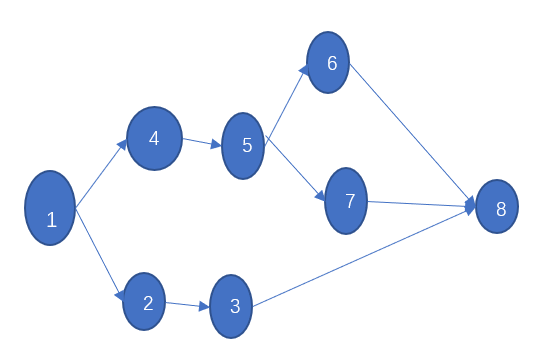
\includegraphics[width=0.66\linewidth,height=0.4\linewidth]{fig/1.jpg}
     	\caption{Poset graph}
     \end{figure}

\blue{All key variables in the pseudo code are normally defined in the main text. Please do so carefully.}

\blue{How much is Alg.1 new? which part is from the book and what have you changed?}

\blue{I would recommend to rewrite Alg.1 after you properly defined the variables.}

 
 \textbf{Example.1}\\
 	Given a LTL formula $\phi=<>( r1 \vee <>(r2 \vee <>(r3 \vee <> r4))) \vee <>( r5 \vee <>(r6 \vee <>(r7 \vee <> r8)))$, we can get a B\"{u}chi automatom $A_\phi$ with 44 states and 439 edges which is too complexity to be drawed into a graph. After trimming the $A_\phi$, we get a much simplified graph $A^-$ as fig.2 showed. And we can find 283 feasible path from initial node to the accept states. Then, using the algorithm.1, we can get the posets which shows the detail very intuitional as the table.1 showed. In the end, we can rebuild a graph of poset to show the relationships between the actions as fig.3 showed.

\blue{``Eventually'' is written as $\Diamond$, ``and'' and ``or'' are $\land$ and $\lor$.}

\blue{As discussed last time, can you improve the alg. to achieve the following:
\begin{itemize}
\item find a path $\mathbf{p}=e_1e_2\cdots e_N$ in NBA during DFS.
\item store it in $\mathcal{P}=\{\mathbf{p}\}$.
\item use other already-found paths in $\mathcal{P}$ to determine the poset \emph{specifically} for $\mathbf{p}$.
\end{itemize}
This would be an \emph{anytime} algorithm, which is asymptotically complete as time goes to infinity.
The benefit is that you do not need to find all simple paths in NBA in one shot. 
}

\textbf{Remark.1} \\
	 The reason why make a map from a actions path $l_a$ to a sequence from $1$ to $n$ is to avoid the interference with the same action.
	  Once the actions $\alpha$ and $\beta$ existed in the $l_a$ more than twice, we may found that the $\alpha||\beta$ while $\alpha<\beta$ at the same time.

\blue{What is this map? your explanation sounds like a direct enumeration.}
  
\textbf{To be proved} \\
	We need to proved that, once get a feasible path in $L_a$, can find all other path stand for the same . for any path 
  
 	
 	\begin{figure}[htp]
 		\centering
 		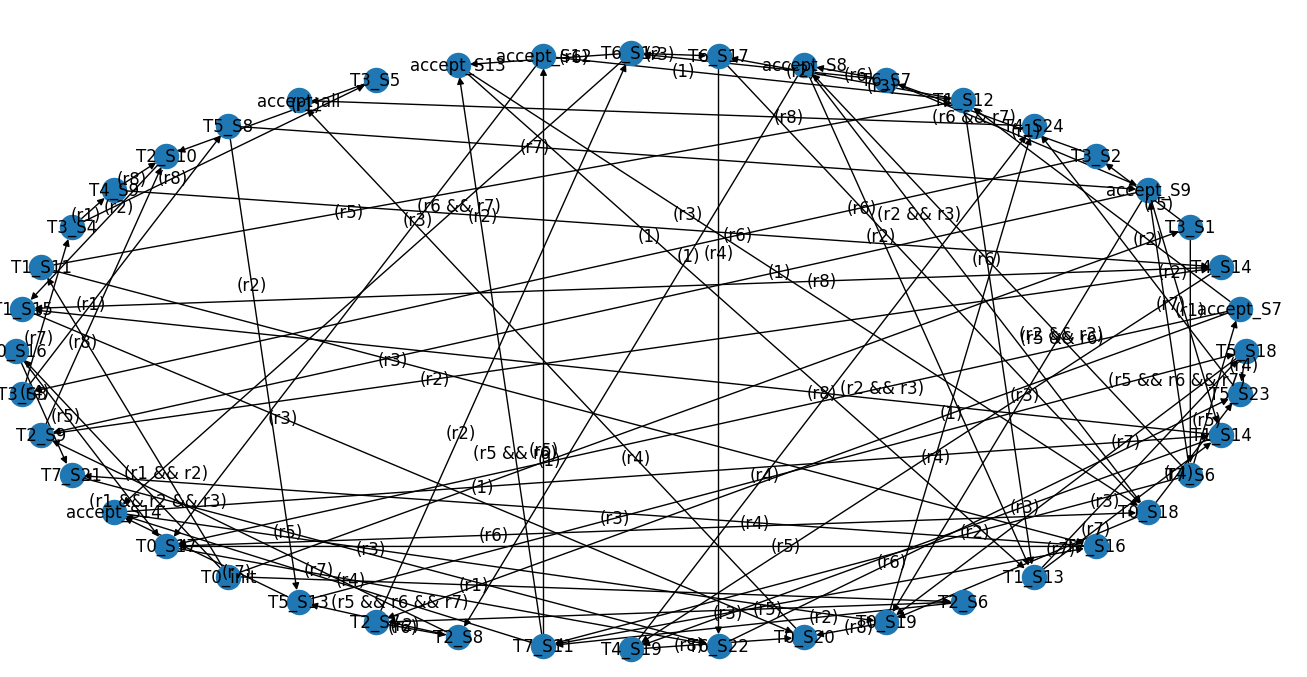
\includegraphics[width=0.66\linewidth,height=0.4\linewidth]{fig/2.jpg}
 		\caption{Trimmed NBA graph}
 	\end{figure}
 
 \begin{table}[]
 	\caption{Poset}	
 	\begin{tabular}{cllll}
 		\cline{1-2}	
 		
 		\multicolumn{1}{|c|}{parallel}    & \multicolumn{1}{l|}{(0,1),(0,5),(0,6),(0,7),(1,2),(1,3),(1,4),(2,5),(2,6),(2,7),(3,5),(3,6),(3,7),(4,5),(4,6),(4,7)} &  &  &  \\ \cline{1-2}
 		\multicolumn{1}{|c|}{less\_than}  & \multicolumn{1}{l|}{(0, 2), (1, 5), (2, 3), (3, 4), (5, 6), (6, 7)}                                                  &  &  &  \\ \cline{1-2}
 		\multicolumn{1}{|c|}{action\_map} & \multicolumn{1}{l|}{{[}'(r1)','(r5)','(r2)','(r3)','(r4)','(r6)','(r7)','(r8)'{]}}                                   &  &  &  \\ \cline{1-2}
 		&                                                                                                                      &  &  & 
 		
 	\end{tabular}





 \end{table}	
 	\begin{figure}[htp]
	\centering
	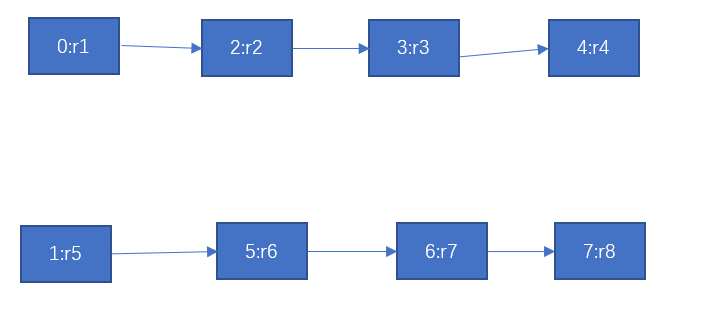
\includegraphics[width=0.66\linewidth,height=0.4\linewidth]{fig/3.jpg}
	\caption{Poset graph}
\end{figure}
\end{document}
